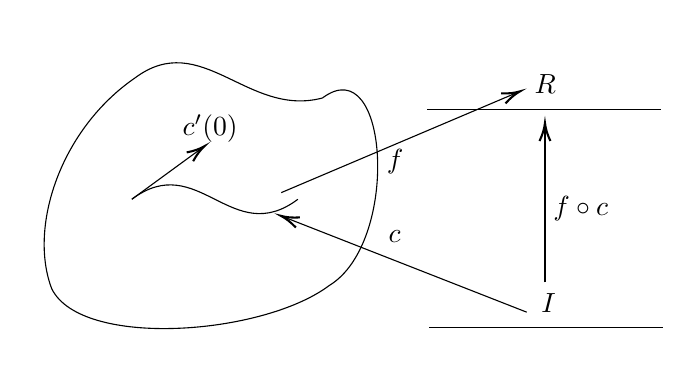
\begin{tikzpicture}[x=0.75pt,y=0.75pt,yscale=-0.8,xscale=0.8]
%uncomment if require: \path (0,300); %set diagram left start at 0, and has height of 300

%Curve Lines [id:da014063753011146707] 
\draw    (103.8,187) .. controls (89.6,150) and (108.8,91) .. (153.8,60) ;
%Curve Lines [id:da6854687890121294] 
\draw    (153.8,60) .. controls (193.8,30) and (221.8,84) .. (266.8,72) ;
%Curve Lines [id:da8800895461125313] 
\draw    (103.8,187) .. controls (121.8,223) and (230.8,215) .. (270.8,185) ;
%Curve Lines [id:da9135462557807166] 
\draw    (266.8,72) .. controls (306.8,42) and (313.8,159) .. (270.8,185) ;
%Curve Lines [id:da6496864524155734] 
\draw    (152,133) .. controls (192,103) and (212,163) .. (252,133) ;
%Straight Lines [id:da4417753278815133] 
\draw    (152,133) -- (194.19,102.18) ;
\draw [shift={(195.8,101)}, rotate = 143.85] [color={rgb, 255:red, 0; green, 0; blue, 0 }  ][line width=0.75]    (10.93,-3.29) .. controls (6.95,-1.4) and (3.31,-0.3) .. (0,0) .. controls (3.31,0.3) and (6.95,1.4) .. (10.93,3.29)   ;
%Straight Lines [id:da5936473075833075] 
\draw    (331,210) -- (471.8,210) ;
%Straight Lines [id:da027889446822472186] 
\draw    (330,79) -- (470.8,79) ;
%Straight Lines [id:da6293384131482878] 
\draw    (389.8,201) -- (243.66,143.73) ;
\draw [shift={(241.8,143)}, rotate = 21.4] [color={rgb, 255:red, 0; green, 0; blue, 0 }  ][line width=0.75]    (10.93,-3.29) .. controls (6.95,-1.4) and (3.31,-0.3) .. (0,0) .. controls (3.31,0.3) and (6.95,1.4) .. (10.93,3.29)   ;
%Straight Lines [id:da21227327133603646] 
\draw    (242,129) -- (383.96,68.78) ;
\draw [shift={(385.8,68)}, rotate = 157.01] [color={rgb, 255:red, 0; green, 0; blue, 0 }  ][line width=0.75]    (10.93,-3.29) .. controls (6.95,-1.4) and (3.31,-0.3) .. (0,0) .. controls (3.31,0.3) and (6.95,1.4) .. (10.93,3.29)   ;
%Straight Lines [id:da2883428159096417] 
\draw    (400.8,183) -- (400.8,89) ;
\draw [shift={(400.8,87)}, rotate = 90] [color={rgb, 255:red, 0; green, 0; blue, 0 }  ][line width=0.75]    (10.93,-3.29) .. controls (6.95,-1.4) and (3.31,-0.3) .. (0,0) .. controls (3.31,0.3) and (6.95,1.4) .. (10.93,3.29)   ;

% Text Node
\draw (397,188.4) node [anchor=north west][inner sep=0.75pt]    {$I$};
% Text Node
\draw (393,56.4) node [anchor=north west][inner sep=0.75pt]    {$\mathbb{R}$};
% Text Node
\draw (305,150.4) node [anchor=north west][inner sep=0.75pt]    {$c$};
% Text Node
\draw (304,101.4) node [anchor=north west][inner sep=0.75pt]    {$f$};
% Text Node
\draw (181,80.4) node [anchor=north west][inner sep=0.75pt]    {$c'( 0)$};
% Text Node
\draw (404.3,129.4) node [anchor=north west][inner sep=0.75pt]    {$f\circ c$};


\end{tikzpicture}